%% iccp20_template.tex
%% Created by Ayan Chakrabarti from the IEEE bare_jrnl_compsoc.tex file.
%%
%% bare_jrnl_compsoc.tex
%% V1.4b
%% 2015/08/26
%% by Michael Shell
%% See:
%% http://www.michaelshell.org/
%% for current contact information.
%%
%% This is a skeleton file demonstrating the use of IEEEtran.cls
%% (requires IEEEtran.cls version 1.8b or later) with an IEEE
%% Computer Society journal paper.
%%
%% Support sites:
%% http://www.michaelshell.org/tex/ieeetran/
%% http://www.ctan.org/pkg/ieeetran
%% and
%% http://www.ieee.org/

%%*************************************************************************
%% Legal Notice:
%% This code is offered as-is without any warranty either expressed or
%% implied; without even the implied warranty of MERCHANTABILITY or
%% FITNESS FOR A PARTICULAR PURPOSE! 
%% User assumes all risk.
%% In no event shall the IEEE or any contributor to this code be liable for
%% any damages or losses, including, but not limited to, incidental,
%% consequential, or any other damages, resulting from the use or misuse
%% of any information contained here.
%%
%% All comments are the opinions of their respective authors and are not
%% necessarily endorsed by the IEEE.
%%
%% This work is distributed under the LaTeX Project Public License (LPPL)
%% ( http://www.latex-project.org/ ) version 1.3, and may be freely used,
%% distributed and modified. A copy of the LPPL, version 1.3, is included
%% in the base LaTeX documentation of all distributions of LaTeX released
%% 2003/12/01 or later.
%% Retain all contribution notices and credits.
%% ** Modified files should be clearly indicated as such, including  **
%% ** renaming them and changing author support contact information. **
%%*************************************************************************


\documentclass[10pt,journal,compsoc]{IEEEtran}
% \newif\ifpeerreview

%%% Important: for camera ready submissions, replace the following line
%%% with \peerreviewfalse
% \peerreviewfalse


\usepackage[nocompress]{cite}
\usepackage{url}
\usepackage{amsmath,amssymb,graphicx}

\usepackage{lipsum} % Only used to generate random text.


\usepackage[switch]{lineno}

\usepackage{hyperref}

\usepackage{array}
\newcolumntype{M}[1]{>{\centering\arraybackslash}m{#1}}

% Insert your paper ID and information below
% \newcommand{\paperID}{XXXX}

% Enter your paper title below
\title{Synthesis of brain tumor MRI images using GAN aggregation with style transfer}

% Enter your author information before
% Note this is only necessary for the camera review. Submissions are anonymized.
\author{Sarah Hindawi,
        Suman Bagri,
        Vignesh Edithal% <-this % stops a space
% \IEEEcompsocitemizethanks{\IEEEcompsocthanksitem M. Shell is with the Department
% of Electrical and Computer Engineering, Georgia Institute of Technology, Atlanta,
% GA, 30332.\protect\\
% % note need leading \protect in front of \\ to get a newline within \thanks.
% E-mail: see http://www.michaelshell.org/contact.html
% \IEEEcompsocthanksitem J. Doe is with Anonymous University.}% <-this % stops an unwanted space
}


\begin{document}

\IEEEtitleabstractindextext{%
\begin{abstract}
Tumor classification and detection are critical for a quick and effective cure. This motivates the idea of developing an automated deep learning (DL) method for classification of brain tumor images. However, DL has raised concerns regarding invading patients' privacy. Also, it is expensive and time-intensive to collect large amounts of MRI images. In addition, many medical imaging datasets are imbalanced which makes it harder for the model to detect outliers. Hence, data augmentation is a crucial necessity in medical image analysis. Traditional data augmentation methods such as rotation, scale, crop, etc. create highly correlated images and lack of variance which prevents any DL model from learning the underlying feature of the image. Meanwhile, Generative Adversarial Networks (GAN) have shown promising results in generating synthetic data with good generalization ability to large image datasets. GANs also serve as an anonymization tool which reduces data handling costs. In this work, we use the Aggregation GAN (AGGrGAN) \cite{Mukherkjee2022} model to capture both the unique features and localized information of a source image using style transfer and also the shared information among the different latent representations of multiple images using multiple GANs. We apply style transfer after aggregation to increase resemblance to the original images. Then, we perform an ablation study of aggregation and style transfer to evaluate their impact on performance. Finally, we train a classification network to study the impact of injecting fake images into the training dataset on the performance of the classifier, this also allows us to evaluate the images qualitatively. We make our code available at \url{https://github.com/edithal-14/csc2529-2022-project}.
\end{abstract}

\begin{IEEEkeywords} % Enter keywords here
GAN, MRI, Brain, Tumor, Style Transfer, Aggregation, DCGAN, WGAN, UNet, Data Augmentation
\end{IEEEkeywords}
}


% Make Title
% \ifpeerreview
% \linenumbers \linenumbersep 15pt\relax 
% \author{Paper ID \paperID\IEEEcompsocitemizethanks{\IEEEcompsocthanksitem This paper is under review for ICCP 2020 and the PAMI special issue on computational photography. Do not distribute.}}
% \markboth{Anonymous ICCP 2020 submission ID \paperID}%
% {}
% \fi
\maketitle



% The first section title should be wrapped inside a \IEEEraisesectionheading as follows.
\IEEEraisesectionheading{
  \section{Introduction}\label{sec:introduction}
}
% The very first letter of the paper is a 2 line initial drop letter
% followed by the rest of the first word in caps.
% 
% form to use if the first word consists of a single letter:
% \IEEEPARstart{A}{demo} file is ....
% 
% form to use if you need the single drop letter followed by
% normal text (unknown if ever used by the IEEE):
% \IEEEPARstart{A}{}demo file is ....
% 
% Some journals put the first two words in caps:
% \IEEEPARstart{T}{his demo} file is ....
% 
% Here we have the typical use of a "T" for an initial drop letter
% and "HIS" in caps to complete the first word.


\IEEEPARstart{B}{rain} tumor identification is crucial to prevent long term disabilities. Severe cases such as High Grade Glioma may be fatal. Magnetic Resonance
Imaging (MRI) is a powerful non-invasive tool for obtaining these brain scans. MRI scans can provide key information such as the location, shape, size and the growth
stage of the brain tumor. To perform any medical image analysis using deep learning techniques, a sufficient volume of data with variability is required.
However, traditional image augmentation methods such as scale, rotation, crop etc. create highly correlated images which are unable to capture the underlying features
of the source images. In addition, they might change the pattern useful for diagnosis. Class imbalance is another reason to apply augmentation. Generative Adversarial
Network (GAN) models have shown promising results in generating synthetic data with good generalization ability to large datasets. In this work we use the Aggregation
GAN (AGGrGAN) model to capture both the unique features and localized information of a source image using style transfer and also the shared information
among the different latent representation of multiple images. We then perform an ablation study to quantitatively evaluate (using PSNR and SSIM scores) the generated
images and also to study the impact of aggregation followed by style transfer. For a qualitative analysis, we train a classification network using both real images and
a mixture of real and fake images to study the effectiveness of the images generated by our models. All our experiments have been performed on the BraTS 2020 dataset
\cite{Bakas2017} \cite{Menze2015} \cite{DBLP:journals/corr/abs-1811-02629}. We start off with a literature study of related works in the next section. Then, we describe
the BraTS 2020 dataset and explain the data pre-processing steps in detail. In the methodology section, we explain in brief the internal working of a GAN model as described
in \cite{Goodfellow2014}, then we move on to describing various GAN architectures such as DCGAN \cite{Radford2015}, WGAN \cite{Arjovsky2017}, UNet GAN \cite{Schonfeld2020}.
We also explain the aggregation logic used in AGGrGAN and provide details of the style transfer technique. The last section contains detailed quantitative/qualitative analysis followed by some concluding remarks.

\section{Related Work}

Han et al. \cite{Han2018} have applied DCGAN and WGAN separately on the BraTS 2016 dataset to generate artificial MRI scans. To validate their results, they conducted the
Visual Turing test with 53\% accuracy for WGAN. Nie et al. \cite{Nie2018} have used Fully Convolution Network (FCN) as generator and a basic CNN as the discriminator,
they have proposed 3D FCN to estimate target image from the corresponding source image, they have used ADNI dataset and have obtained a mean PSNR of 34.1. Emami et al.
\cite{Emami2018} have proposed a GAN based model where ResNet is used as the generator and discriminator is a CNN with five convolutional layers which classify the image
as real or fake, they achieved a mean PSNR of 26.6 $\pm$ 1.2 for an IRB approved dataset. Shin et al. \cite{Shin2016} segmented the overall scans of Alzheimer's Disease
Neuroimaging Initiative (ADNI) \cite{Petersen2009} dataset and BraTS dataset into brain anatomy and tumors using pix2pix GAN \cite{Isola2016}. They have obtained the augmented scans by applying different combinations of the segmented brain anatomy and tumor labels by introducing some alternations. Sarkar et al. \cite{Sarkar2020} created
a CNN model to detect the type of brain tumor using MRI scans to classify meningioma, glioma and pituitary tumors.

\section{Methodology}

\subsection{Dataset description}

We use BraTS 2020 dataset for all our experiments. It consists of four MRI modality classes namely, T1 weighted images (T1), Post contrast T1 weighted images (T1ce),
T2 weighted images (T2) and T2 Fluid Attenuated Inversion Recovery (T2-FLAIR). These samples have been acquired with different clinical protocols and various scanners
from multiple institutions. Training data contains a total of 369 NIfti files for each class and testing data contains 125 Nifti files for each class. A Nifti file
corresponds to a 3D image acquired by a MRI scan. The middle layer of the 3D image is chosen for all experiments since that is the biggest in size and contains more
details as compared to rest of the slices which are smaller in size. Each image has a resolution of 240 x 240 pixels. However, due to limited resources at our disposal
we chose to resize the image to 64 x 64 pixels resolution for all our experiments. This also helps with training the GAN model as explained in the later sections.
Sample images from the dataset are shown in Table \ref{table:1}.

\begin{table}[!t]
\renewcommand{\arraystretch}{1.3}
\centering
\caption{Sample images from BraTS 2020 dataset where each row represents a class modality}
\label{table:1}
\begin{tabular}{ M{1cm} M{2cm}  M{2cm}  M{2cm} }
T1 & 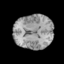
\includegraphics[width=2cm, height=2cm]{t1_1.png} & 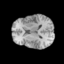
\includegraphics[width=2cm, height=2cm]{t1_2.png} & 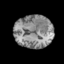
\includegraphics[width=2cm, height=2cm]{t1_3.png} \\
T1ce & 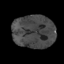
\includegraphics[width=2cm, height=2cm]{t1ce_1.png} & 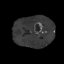
\includegraphics[width=2cm, height=2cm]{t1ce_2.png} & 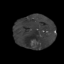
\includegraphics[width=2cm, height=2cm]{t1ce_3.png} \\
T2 & 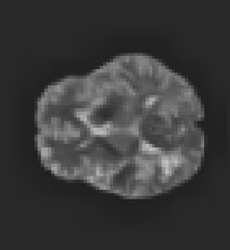
\includegraphics[width=2cm, height=2cm]{t2_1.png} & 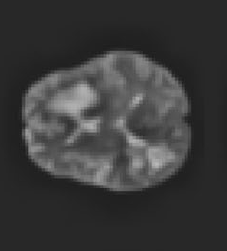
\includegraphics[width=2cm, height=2cm]{t2_2.png} & 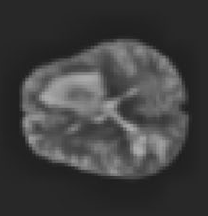
\includegraphics[width=2cm, height=2cm]{t2_3.png} \\
T2-FLAIR & 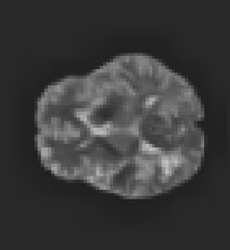
\includegraphics[width=2cm, height=2cm]{t2_1.png} & 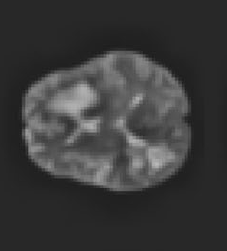
\includegraphics[width=2cm, height=2cm]{t2_2.png} & 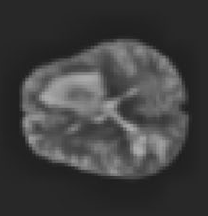
\includegraphics[width=2cm, height=2cm]{t2_3.png} \\
\end{tabular}
\end{table}

\subsection{A brief introduction to Generative Adversarial Network (GAN)}

GAN is a deep learning (DL) framework to capture the distribution of training data such that we can generate new data from that distribution. They were first described 
in \cite{Goodfellow2014}. They consist of two competing models namely Generator and Discriminator. The job of the Generator is to spawn "fake images" that look like the
training images. The job of the Discriminator is to classify whether a given image is real or fake. During training both the model compete in a game with each other to minimize their losses. The equilibrium of the game is when the Generator produces perfect "fake images" and the Discriminator is left to always guess at 50\% probability.

Before we formally define the losses of both the models in a GAN, we would like to mention some notation. Let, $x$ be the data representing an image, $\rho_{data}$ represents the training distribution, $\rho_{latent}$ represents the latent distribution. The output of Discriminator $D(x)$ is the probability of the given image being
real. The output of the Generator $G(z)$ is a fake image where $z$ is the latent distribution of the training distribution. So, $D(G(z))$ is the probability of a
generated image ("fake image") being classified as real. As described in \cite{Goodfellow2014}, $D$ and $G$ play a \textbf{minmax} game where $D$ tries to \textbf{maximize}
the probability that it classifies correctly $\log(D(x))$. $G$ tries to \textbf{minimize} the probability that $D$ will predict its output to be fake $\log(1 - D(G(z)))$.
From the paper, the GAN loss function is described as follows.

% & indicates alignment point
\begin{align*}
  \label{align*:1}
  & min_{G}max_{D} V(D, G) = \\
  \mathbb{E}_{x \sim \rho_{data}(x)} [\log D(x)] & + \mathbb{E}_{z \sim \rho_{latent}(z)} [\log (1 - D(G(z)))]
\end{align*}


In theory the solution to this game is where $\rho_{real} = \rho_{fake}$, however, in practice this is rarely achieved, this makes training a GAN an inherently difficult task. The convergence of GANs is still an active area of research.

\subsection{AGGrGAN model}

The aggregation GAN (AGGrGAN) model as described in \cite{Mukherkjee2022} consists of two different Deep Convolutional GANs (DCGANs) and one Wasserstein GAN (WGAN).
The different DCGAN differ in the way the latent vector is up-sampled to generate the fake image, one uses transposed convolution layers and the other one an explicit
up-sampling operation. The images from each of the GANs are merged together using a weighting scheme which is based on edge detection and PSNR/SSIM metrics. To further
increase the quality of the images, style transfer technique is applied to the output of each GAN and the aggregated image. The architectural diagram of this model is presented in Figure \ref{figure:1}. In the upcoming sections we talk about each of these components in detail.

\begin{figure}[h]
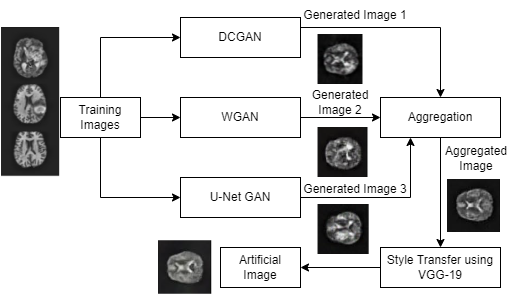
\includegraphics[scale=0.5]{AggrGAN_architecture.png}
\caption{Architecture diagram of Aggregate GAN (AGGrGAN)}
\label{figure:1}
\end{figure}

\pagebreak

\subsection{DCGAN model}

DCGAN was introduced in \cite{Radford2015}, it is an extension of the GAN model described above where Convolutional and Transposed Convolutional layers are used repeatedly
in the Discriminator and Generator model respectively. The Discriminator uses strided convolutional layers to repeatedly downsample the image to a scalar value, it is
suggested to use strided convolution instead of max/mean pooling layer since the former allows the model to learn the downsampling operation suitable for the given data.
The Generator uses strided transposed convolutional layers to repeatedly upscale the latent vector (noise sampled from a multivariate normal distribution) to generate a
"fake image". Both the models use Batch Normalization (BatchNorm) layers to regulate gradients. The Generator and Discriminator use ReLU and Leaky ReLU activation functions
respectively, LeakyReLU helps in healthy flow of gradients across the network and prevents issues such as vanishing gradient problem.

The Generator uses 5 layers of transposed convolutional layers interspersed with BatchNorm and ReLU layers to upsample a latent vector of size 128 to a single channel
64 x 64 image, it uses Tanh layer as the last layer for output. The Discriminator uses 5 layers of convolutional layers interspersed with BatchNorm and Leaky ReLU layers to
downsample the 64 x 64 image into a scalar value, it uses Sigmoid layer as the final layer to output a scalar probability value.

DCGAN is trained using a Binary Cross Entropy (BCE) loss where the ground truth $y$ value for real image is 1 and fake image is 0, this allows us to choose between two different log values in the BCE loss.

\begin{align}
  l_n = - ((y_n * \log x_n) + (1 - y_n) * \log (1 - x_n))
\end{align}

The Discriminator loss is calculated in two steps. First, we feed forward the Discriminator with real images and use $y = 1$ to calculate BCE loss. Then we create a fake
image using feed forward of Generator which is fed to the Discriminator and BCE loss is calculated using $y = 0$. The sum of these losses is the Discriminator loss.
The Generator loss is calculated by creating a fake image using feed forward of Generator, then passing it through Discriminator where the BCE loss is calculated using
$y = 1$. At the end of every mini batch (batch size = 128) the optimizer step is performed (Adam with beta1 = 0.5 and lr = 2e-4). We perform a total of 500 epochs on the training data (369 images) of each modality. The Discriminator loss, Generator loss, mean PSNR and SSIM scores of each mini batch is stored for plotting to visualize the
training process.

\subsection{WGAN model}

Wasserstein GAN proposed by \cite{Arjovsky2017} is an extension of GAN which improves training stability and uses a loss function which is more indicative of the quality
of generated images. It uses a Discriminator (called Critic in WGAN) which outputs different score for real and fake images instead of a probability value. This change
is motivated by the fact that Generator should seek a minimization of Earth Movers (EM) distance between the observed distribution and generating distribution. EM distance
is chosen since it produces large gradients even for large difference in the observed and generated distributions. The Discriminator loss in this case is the negation of 
difference between the critic scores of real and fake images. The Generator loss is the negation of the critic score of fake images. It is to be noted that when training 
WGAN the generator model is updated only one time per $n_critic$ (5 in our case) updates of the critic model. Following is the equation of critic loss in WGAN. 

\begin{align}
  W(P_r, P_{\theta}) = sup_{\Vert f \Vert_{L} \leq 1} \mathbb{E}_{x \sim P_r} [f(x)] - \mathbb{E}_{x \sim P_{\theta}} [f(x)]
\end{align}

Here $sup$ is the least upper bound and $f$ is a 1-Lipschitz function following the constraint.

\begin{align}
  \Vert f(x_1) - f(x+2) \Vert \leq \Vert x_1 -x_2 \Vert
\end{align}

We use two different WGANs based on how the 1-Lipschitz constrained function is implemented. In the WGAN model, we use clip the weights of the critic between -0.01 and 0.01.
However, the WGAN paper suggests that this is not the best way to enforce the 1-Lipschitz constraint. In the WGAN-GP (WGAN Gradient Penalty) model, we add a penalty term to
the critic loss based on how much the second norm of the gradient moves away from 1. The gradient is calculated at an interpolated point which lies between observed and
generated distributions. It is suggested not to used BatchNorm layers when using gradient penalty.

\begin{align}
  W(P_r, P_{\theta}) += \lambda * \mathbb{E}_{\hat{x} \sim P_{\hat{x}}} [(\nabla_{\hat{x}} D(\hat{x}) - 1)^2]
\end{align}

Here $\lambda$ is the regularization parameter which is set to 10 in our case and $\hat{x}$ is the interpolated point.

For the training of WGAN and WGAN-GP we use image size of 64 x 64 pixels resolution and latent vector size of 128. We run 500 epochs with a batch size of 32 with lr = 1e-3 
and beta1 parameter of Adam optimizer set to 0.5

\begin{figure*}[h]
\centering
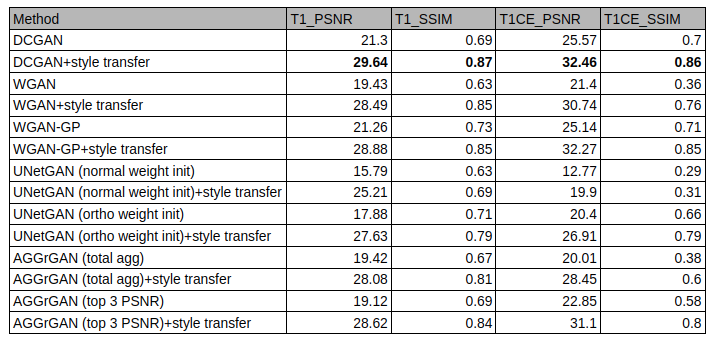
\includegraphics[width=18cm, height=10cm]{score_table.png}
\caption{
  Ablation study showing the effectiveness of aggregation and style transfer. Without the style transfer the order of performance that we get is DCGAN $>$
  WGAN-GP $>$ WGAN $>$ AGGrGAN $>$ UNet GAN (orthonormal weights) $>$ UNet GAN (normal weights). The impact of style transfer seems to be significant.
  In the case of DCGAN it led to a PSNR increase of 8 points and SSIM increase of nearly 0.2 points.
}
\label{figure:3}
\end{figure*}

\subsection{U-Net GAN}
One of the major challenges for GANs is the ability to produce locally and globally coherent images \cite{Schonfeld2020}. In order to tackle this problem, the authors of \cite{Schonfeld2020} proposed a modification to the "vanilla" GAN where the standard classification network used as a discriminator ($D$) was replaced with an encoder-decoder framework of a U-Net. In an encoder-decoder network, the encoder acts as a classification network that downsamples the input capturing global image context which is then fed into a bottleneck layer. The decoder, subsequently, upsamples the output of the bottleneck by accommodating encoder output at each level using skip-connections thus learning locally-relevant details. A U-Net classifier also specializes in providing state-of-the-art results while requiring only a few training images to learn. It does so by using each training image efficiently to learn a more precise segmentation map.

Our implementation of the U-Net GAN differs from \cite{Schonfeld2020} in two main areas: \\
\underline{Architecture:}

We use a standard U-Net architecture (as described in \cite{unet}) as base for the Discriminator($D^U$) with a few modifications. First, we use Leaky ReLU (with negative slope $= 0.2$) as activation functions between convolutional layers. Second, for down-sampling (in the encoder), we use average pooling with a $2 \times 2$ kernel size. Third, for up-sampling (in the decoder), we use transposed convolutional layers with a $2 \times 2$ kernel size and a stride of 2. Finally, we use a convolutional layer with a $24 \times 24$ kernel size which produces a singular value for $64 \times 64$ input image size. This is, subsequently passed through a sigmoid activation function to give a probabilistic value indicating real/fake image. As part of our exploratory study, we also used 2 different weight initialization methods for the Discriminator: Normal(sampled from $\mathcal{N}(0,0.02)$) and Orthogonal (as described in \cite{ortho}). The Generator($G^U$) architecture is exactly the same as that for DCGAN. \\
\underline{Training:}

We adopt a training methodology similar to that for DCGAN. The BCE loss is used to train both the $G^U$ and the $D^U$ as described in 3.4. Training is done for 1000 epochs with a batch size of 128. Adam optimizer with beta1=0.5, beta2=0.999 and lr=2e-4 is used for both $G^U$ and $D^U$.

The main reason behind using a different U-Net GAN architecture than \cite{Schonfeld2020} was to keep the training process same for all the GANs. However, it is worthwhile to note that this architecture may not result in the best possible synthetic image generation in terms of evaluation metrics as this architecture does not make use of the per-pixel outputs from the Discriminator to train the Generator but rather combines them to produce a singular value (fake/real input image) to compute the Generator loss.

\subsection{Aggregation}

From the set of 5 (1 DCGAN + 2 WGAN + 2 UNet GAN) fake images generated, we choose the top 3 images based on SSIM/PSNR as suggested by \cite{Mukherkjee2022}, aggregation
algorithm is then run on these images. Firstly, we apply a Sobel filter to produce edge mapped images, then a Gaussian filter is applied to smooth the edges (we found
sigma = 2 to be the best for this purpose). Then, the images are weighted based on the value of this smoothened edge mapped image. Finally a weighted addition of the images
is carried out to generate the aggregated images. We also experimented with a PSNR/SSIM metric based weighting scheme but found the results to be similar to that of the
above. In the aggregation algorithm proposed in \cite{Mukherkjee2022}, they only chose top 2 out of 3 fake images based on PSNR/SSIM metrics. However, we experimented with 
an ablation study of removing this top $n$ selection component by performing aggregation across all the images. As mentioned in the result and analysis section this proved to be not very effective.

\subsection{Style Transfer}

We apply style transfer to the output of GAN models to improve the resemblance of synthetic images with respect to the real images. We use a pre-trained VGG-19 model (pre-trained on ImageNet) to extract style and content features of the image. The synthetic image is passed through the intermediate layers 0, 5 and 10 of the VGG-19 model and the resulting output is used to calculate the total loss which is a linear combination of style loss (weight = 10, alpha) and content loss (weight = 5, beta). The parameters alpha and beta can be tuned to control the degree of similarity. The total loss is minimized by an Adam optimizer with beta1 = 0.9 and beta2 = 0.999. The content image (fake image) and the style image (fake image) is given to the model and the optimizer updates the content image to minimize the total loss every epoch. We used 500 epochs for the style transfer process. 

\subsection{Classifier model}

To classify the images as either T1 or T1ce class, we used a classification model which
consists of 2D convolution, ReLU and max pooling layers. We use 2 blocks each consisting of 2 Conv2D layers followed by a ReLU and a max pooling layer. Finally we flatten the output and pass it through 2 consecutive linear layers. We used cross entropy loss for training the model. We chose a batch size of 256, image size of 64. We used Adam optimizer with learning rate of 1e-3 for 15 epochs for all the cases. Our case study was performed on 5 different proportions of real data and fake data which we used to train the model. These
4 cases are explained in detail in the next section.

\section{Results and Analysis}

\subsection{Evaluation metrics: SSIM and PSNR}

To quantitatively evaluate our approach we use Peak Signal to Noise Ratio (PSNR) and Structural Similarity Index Measure (SSIM). We use these metrics to evaluate the
performance of each of the individual GANs and the aggregated image. These metrics are also used to evaluate the performance after style transfer. We now formally define
these metrics

\textbf{PSNR}: It denotes the ratio of maximum intensity value and present noise value. Maximum intensity in our images is 255 and the square root of the Mean Squared
Error (MSE) can be used to measure noise. Therefore, PSNR is evaluated as follows:

\begin{align}
  PSNR = 20 \log_{10} MAX_f / \sqrt{MSE}
\end{align}

\textbf{SSIM}: It denotes the degree of similarity between two images. The closer the similarity the higher the SSIM. Two identical images have SSIM = 1.
SSIM is evaluated using the following formula

\begin{align}
  SSIM = \frac{(2 \mu_x \mu_y + c_1) (2 \sigma_{xy} + c_2)}{(\mu_x^2 + \mu_y^2 + c_1) (\sigma_x^2 + \sigma_y^2 + c_2)}
\end{align}

Here, $\mu_x$ and $\mu_y$ are the mean intensity value of both the images, $\sigma_x$ and $\sigma_y$ are the standard deviation of the intensity values present in both
the images. $\sigma_{xy}$ is the covariance between the intensities of both the images. $c_1$ and $c_2$ are constants used to negate the weak denominator effect.

\subsection{Generated Images}

We run inference on the model and the trained weights to generate the fake images corresponding to a real image. For every real image we run 100 rounds of inference using
random gaussian latent vectors, then, we select the fake image with the highest PSNR with respect to the real image. Based on our experiments, we got the highest mean PSNR
across all the 369 image pairs for T1 and T1ce classes out of the 4 classes in the BraTS 2020 dataset. Therefore, we only used results for T1 and T1ce for analysis. Figure 
\ref{figure:2} shows sample generated images using individual models and after aggregation for both the classes, note that these are the images after style transfer. Note
that we have upscaled the images in the aforementioned figure from 64 x 64 resolution to 256 x 256 resolution in order to better visualize the differences between images
without the images getting blurred or teared. For this purpose we used the super resolution interface in the cv2 python library, EDSR x4 pretrained model was used with
this interface to upscale the images dimensions by 4 times.

\begin{figure}[h]
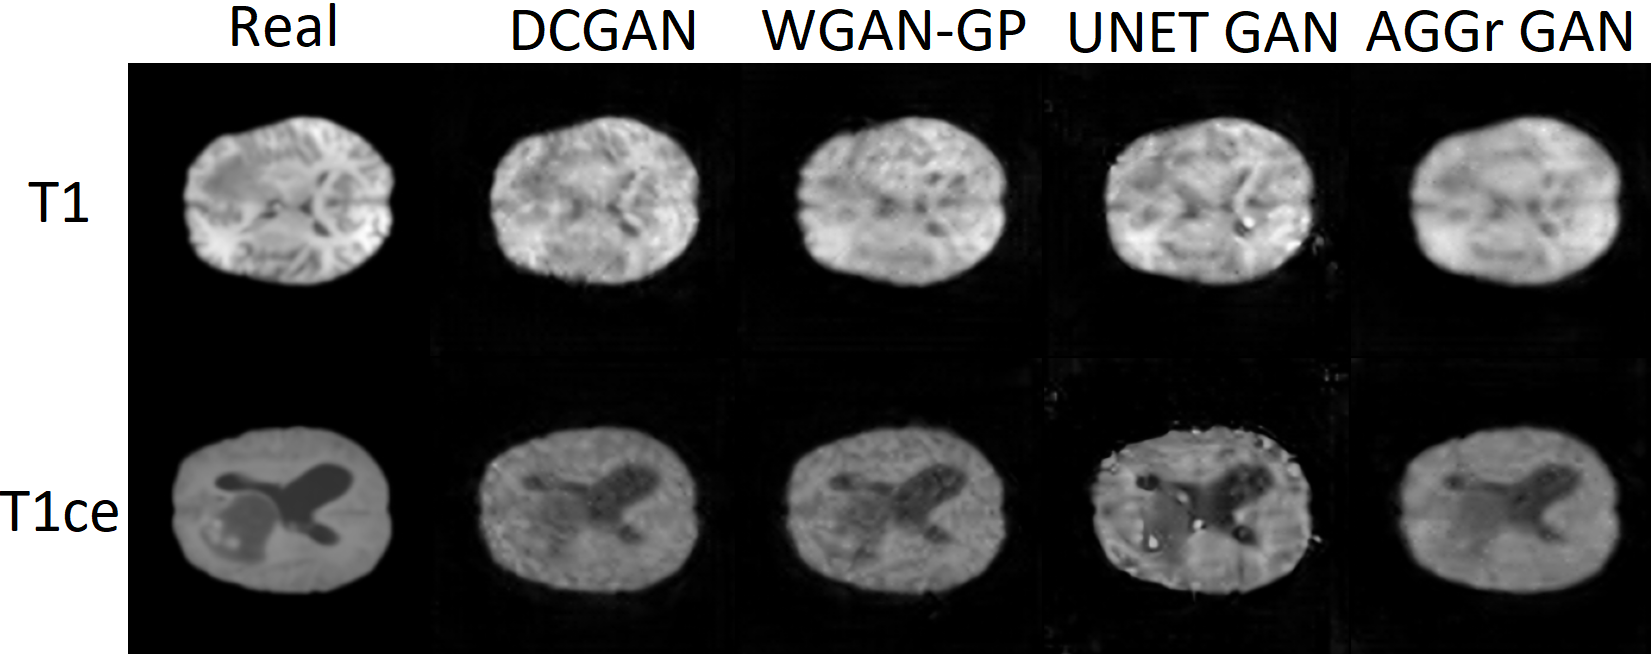
\includegraphics[width=8cm, height=4cm]{upscaled_grid_with_labels.png}
\caption{
  Sample images generated by DCGAN, WGAN-GP, UNet GAN and AGGrGAN and their comparison with the real image. We only used images from T1 and T1ce modality in our experiments. Note that these images are upscaled from 64 x 64 resolution to 256 x 256 resolution using upscaling techniques from cv2 python library.
}
\label{figure:2}
\end{figure}

Figure \ref{figure:3} shows an ablation study of various components of the AGGrGAN model. Quantitatively judging, DCGAN with style transfer seems to be the best performing
model with PSNR = 29.64 and SSIM = 0.87.

\subsection{Training}

In this subsection we analyze the generator and discriminator losses as well as PSNR and SSIM metrics as the model training progresses. We show the graphs for the best
performing model that is DCG    AN. Figure \ref{figure:4} shows the Generator and Discriminator losses as the training proceeds. It is evident that training the Generator of
a GAN is difficult than training the Discriminator since the latter loss is very volatile as compared to the former. The Generator loss first decreases rapidly then
starts decreasing steadily. 

\begin{figure}[h]
\centering
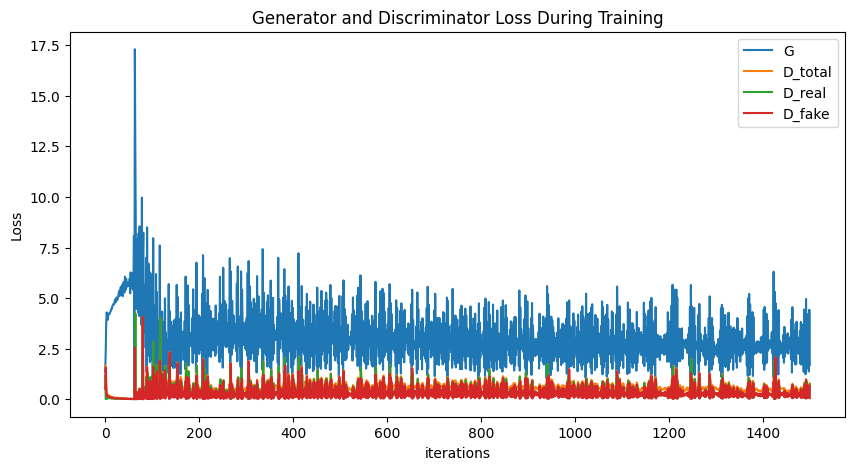
\includegraphics[width=8cm, height=5cm]{gen_disc_loss.png}
\caption{
  Generator and Discriminator losses of DCGAN as training progresses. The blue curve denotes the Generator losses which rapidly decreases at first
  then steadily decreases as the training progresses. The Discriminator loss on the other hand is more or less constant during the training.
}
\label{figure:4}
\end{figure}

The PSNR value trend seems to agree with the above graph, it increases rapidly in the beginning followed by a steady increase as can be seen in Figure \ref{figure:5}

\begin{figure}[h]
\centering
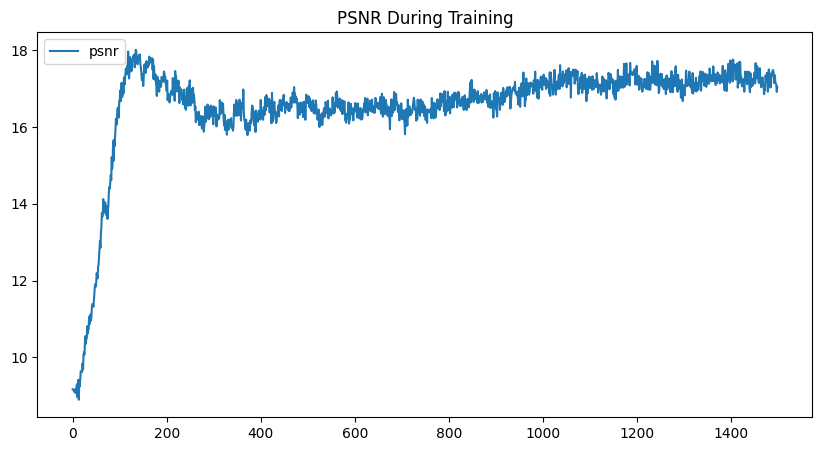
\includegraphics[width=8cm, height=5cm]{psnr.png}
\caption{
  PSNR score of the Generated images during training.
}
\label{figure:5}
\end{figure}

The SSIM scores on the other hand continuously increase at the same rate during training when we ignore the fluctuations caused due to instability in training a GAN.
This can be seen in Figure \ref{figure:6}. These results show that we could have run the DCGAN for more than 500 epochs, however, we couldn't do it due to resource
constraints.

\begin{figure}[h]
\centering
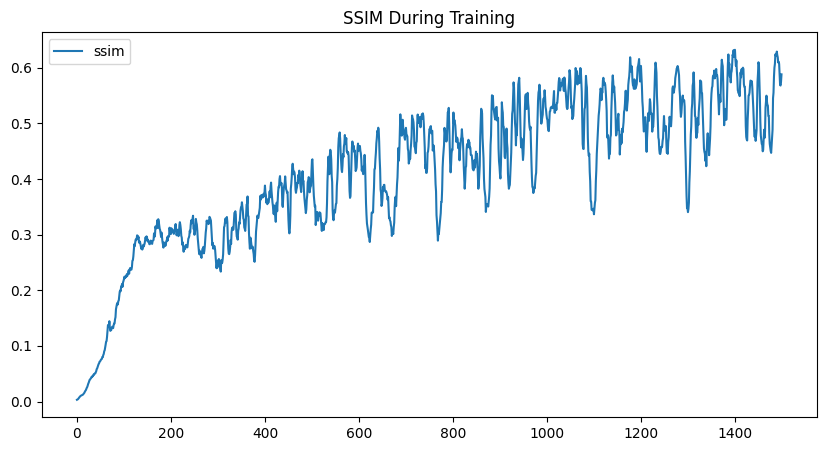
\includegraphics[width=8cm, height=5cm]{ssim.png}
\caption{
  SSIM score of the Generated images during training.
}
\label{figure:6}
\end{figure}

\subsection{Classification using fake images}

We conducted 5 case studies using different proportions of real and fake data for training
the classifier. In each case 50\% of the testing data was used for validation. Note that
since T1 and T1ce images look different from each other (especially in terms of intensity),
most of the cases result in a high accuracy score.

\textbf{Case 1}: We chose 80\% of real images for training and 20\% of real images for
testing. This is our base case where we classified the images with 89.8\% accuracy.

\textbf{Case 2}: We chose 100\% of the fake images produced by WGAN-GP for training and
100\% of real images for testing. We used this setup to qualitatively assess the quality
of the fake images. Classification accuracy was 90.1\% accuracy in this case.

\textbf{Case 3}: We used 50\% of real images and 50\% of fake images for training and
50\% of fake images for testing. This is the most common scenario in the real world where
we would use a mixture of real data with augmented data to boost model performance.
Classification accuracy was 95\% for this case which is considerably higher than Case 1.

\textbf{Case 4}: This is similar to Case 2 with the only change being that we used the
fake images generated by DCGAN instead. Classification accuracy was 90\% in this case which
is approximately the same as Case 2.

\textbf{Case 5}: We made a slight change to Case 1 by additionally adding 100\% of fake
images. This resulted in accuracy of 92\% which is slightly better than Case 1.

We can clearly see that in all the cases adding synthetic images in the training processes
boosts the performance of the classification model.

\section{Conclusion}

In this worked we showed a mechanism to create and aggregated fake image using the output
from various GAN models. This allows us to learn features from the shared space of all the
latent vectors. We explained each GAN model and the aggregation process in detail. We also
performed style transfer on top of the fake images to add more internal details of the brain
to the fake images to further increase the resemblance with the real images which is evident
by a sharp increase in PSNR and SSIM scores. We performed an ablation study to understand
the impact of each part of our workflow. The experimental setup was explained and we showed
that DCGAN with style transfer resulted in the best performance. Finally, we trained a
basic classifier with a mixture of real and fake data and showed the boost in the 
performance of the classification model. Therefore, we quantitatively and qualitatively
evaluated the output of our models and showed that the GANs can produce a good quality
MRI image of a brain tumor. This fake data is useful since there is no associated data 
handling risks.

\bibliographystyle{IEEEtran}
\bibliography{references}

\end{document}